\section{Week 3 - Poisson's and Laplace's Equations}

\subsection{Applications of Vector Calculus to Electrostatics}

The primary goal of electrostatics is to find the electric field $\vb{E}(\vb{r})$ generated by a given stationary charge distribution $\rho(\vb{r}')$. Because charges do not move, Coulomb's law and the superposition principle allow us to express the field directly as:
\begin{equation}
    \vb{E}(\vb{r}) = \frac{1}{4\pi\varepsilon_0}\int \frac{\rho(\vb{r}')}{\gr^2} \vu*{\gr} \dd{V}'
\end{equation}
While exact, this integral formulation presents practical challenges:
\begin{itemize}
    \item The vector integral is generally difficult or impossible to evaluate analytically.
    \item Symmetric problems can often be simplified via Gauss's law, but geometric symmetry is rare in realistic setups.
\end{itemize}

To simplify the mathematics, we introduced the electrostatic scalar potential $\phi(\vb{r})$:
\begin{equation}
    \phi(\vb{r}) = \frac{1}{4\pi\varepsilon_0}\int \frac{\rho(\vb{r}')}{\gr} \dd{V}'
\end{equation}
Working with $\phi(\vb{r})$ provides a clear advantage: it is a scalar function, avoiding component-wise vector integration. However, two major hurdles remain:
\begin{itemize}
    \item The scalar integral can still be analytically intractable.
    \item The source charge distribution $\rho$ may be unknown \emph{a priori} (e.g., on conducting surfaces where charges redistribute freely).
\end{itemize}

An alternative, powerful approach is to recast the problem into differential equations. Starting from Gauss's law in differential form:
\begin{equation}
    \div{\vb{E}} = \frac{\rho}{\varepsilon_0}
\end{equation}
and using the relationship between the electric field and the scalar potential:
\begin{equation}
    \vb{E} = -\grad{\phi}
\end{equation}
substituting $\vb{E}$ into Gauss's law yields:
\begin{equation}
    \div(-\grad{\phi}) = \frac{\rho}{\varepsilon_0} \implies \grad^2\phi = -\frac{\rho}{\varepsilon_0}
\end{equation}

\begin{definition}{Poisson's and Laplace's Equations}{poisson_laplace}
The fundamental second-order partial differential equation governing the electrostatic potential in the presence of a charge density $\rho$ is \textbf{Poisson's equation}:
\begin{equation}
    \grad^2\phi = -\frac{\rho}{\varepsilon_0}
\end{equation}
In regions of space where no free charge is present ($\rho = 0$), this simplifies to \textbf{Laplace's equation}:
\begin{equation}
    \grad^2\phi = 0
\end{equation}
Solutions to Laplace's equation are referred to as \textbf{harmonic functions}.
\end{definition}

\subsubsection*{The Laplacian Operator}

In Cartesian coordinates, the del operator is defined as:
\begin{equation}
    \grad \equiv \left(\pdv{x}, \pdv{y}, \pdv{z}\right) = \vu{x}\pdv{x} + \vu{y}\pdv{y} + \vu{z}\pdv{z}
\end{equation}
The Laplacian is the divergence of the gradient:
\begin{align}
    \grad^2 f \equiv \div(\grad f) &= \left(\vu{x}\pdv{x} + \vu{y}\pdv{y} + \vu{z}\pdv{z}\right) \cdot \left(\pdv{f}{x}\vu{x} + \pdv{f}{y}\vu{y} + \pdv{f}{z}\vu{z}\right) \nonumber \\
    &= \pdv[2]{f}{x} + \pdv[2]{f}{y} + \pdv[2]{f}{z}
\end{align}
The Laplacian is a second-order linear differential operator measuring the local \textbf{curvature} or concavity of a function. In curvilinear coordinates (cylindrical, spherical), metric scale factors introduce extra derivative terms.

\begin{example}[Geometrical Interpretation of the Laplacian]
Consider the paraboloid function:
\begin{equation}
    \phi(x, y) = \frac{a}{4}\left(x^2 + y^2\right)
\end{equation}
Computing its Laplacian gives:
\begin{equation}
    \grad^2\phi = \pdv[2]{\phi}{x} + \pdv[2]{\phi}{y} + \pdv[2]{\phi}{z} = \frac{a}{4}(2 + 2) = a
\end{equation}
The Laplacian directly quantifies the net upwards curvature $a$ of the surface.

\begin{center}
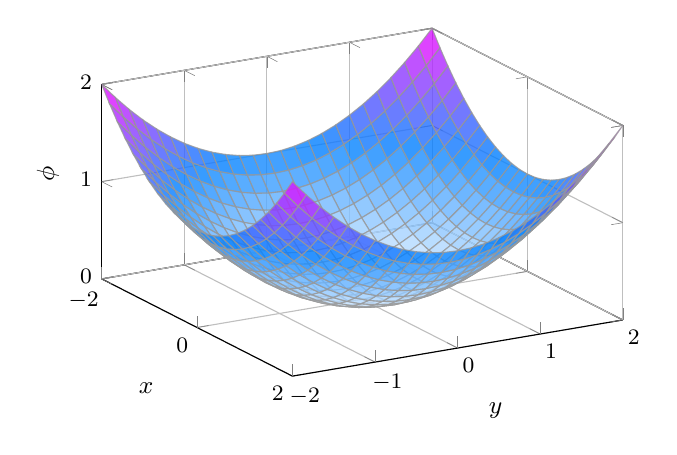
\begin{tikzpicture}
\begin{axis}[
    width=8.2cm,
    height=6cm,
    view={60}{30},
    xlabel={$x$},
    ylabel={$y$},
    zlabel={$\phi$},
    colormap/cool,
    samples=25,
    domain=-2:2,
    domain y=-2:2,
    zmin=0, zmax=2,
    grid=major,
    tick label style={font=\footnotesize},
    label style={font=\small}
]
\addplot3[surf, opacity=0.8, faceted color=black!40] {0.25*(x^2 + y^2)};
\end{axis}
\end{tikzpicture}
\end{center}

When a potential satisfies Laplace's equation ($\grad^2\phi = 0$), its net curvature vanishes everywhere in that region. Consequently, the potential cannot curve upward or downward simultaneously in all directions, meaning $\phi$ \textbf{cannot have local maxima or minima within a charge-free volume}.
\end{example}

% =========================================================================
\subsubsection{Earnshaw's Theorem}
% =========================================================================

\begin{theorem}{Earnshaw's Theorem}{earnshaw}
It is impossible to maintain a charged particle in stable static equilibrium using electrostatic forces alone; that is, the electrostatic potential $\phi$ cannot possess an isolated local minimum (or maximum) in free space.
\end{theorem}

\begin{proofbox}[Proof via Gauss's Law]
We proceed by contradiction. Suppose there exists an electrostatic field $\vb{E}$ capable of holding a positive charge $q > 0$ in stable equilibrium at a point $P$ in an empty region.

For the equilibrium to be stable, any small displacement $\dd{\vb{x}}$ away from $P$ must generate a restoring force pushing the particle back toward $P$. Thus, the electric field $\vb{E}$ must point inward toward $P$ from all directions.

\begin{center}
\begin{tikzpicture}[scale=1.1, >=Stealth]
    % Central point P
    \coordinate (P) at (0,0);
    \draw[fill=ThmColor] (P) circle (2.2pt) node[below right] {$P$};

    % Small Gaussian sphere
    \draw[dashed, thick, DefColor] (P) circle (1.4cm);
    \node[DefColor, above right] at (45:1.4) {$S$};

    % Inward electric field vectors
    \foreach \ang in {0, 45, 90, 135, 180, 225, 270, 315} {
        \draw[->, thick, ExColor] (\ang:1.9) -- (\ang:1.45);
        \node[font=\footnotesize, ExColor] at (\ang:2.1) {$\vb{E}$};
    }
\end{tikzpicture}
\end{center}

Construct a small spherical surface $S$ centered at $P$. Because $\vb{E}$ points inward everywhere on $S$, the scalar product $\vb{E} \cdot \dd{\vb{a}} < 0$ over the entire surface, yielding a strictly negative net flux:
\begin{equation}
    \oint_S \vb{E} \cdot \dd{\vb{a}} < 0
\end{equation}
However, Gauss's law demands:
\begin{equation}
    \oint_S \vb{E} \cdot \dd{\vb{a}} = \frac{Q_{\text{enc}}}{\varepsilon_0}
\end{equation}
Because the region contains no source charges ($Q_{\text{enc}} = 0$), the total flux must be zero, directly contradicting the inward-flux requirement. Hence, an electrostatic field cannot hold a charge in stable static equilibrium.
\end{proofbox}

\subsubsection*{Physical Domains of Laplace's Equation}

Laplace's equation $\grad^2\phi = 0$ is ubiquitous across physics:
\begin{itemize}
    \item \textbf{Steady-state heat conduction:} $\grad^2 T = 0$ (Fourier's law with no internal sources).
    \item \textbf{Static membrane deflection:} $\grad^2 z = 0$ (small transverse displacements).
    \item \textbf{Fluid dynamics:} $\grad^2 \psi = 0$ (potential flow for incompressible, irrotational fluids).
    \item \textbf{Electrostatics:} $\grad^2\phi = 0$ in vacuum.
\end{itemize}

\subsubsection*{Properties in 1D, 2D, and 3D}

\paragraph{One-Dimensional Case.}
In 1D, Laplace's equation reduces to an ordinary differential equation:
\begin{equation}
    \dv[2]{\phi}{x} = 0 \implies \phi(x) = mx + b
\end{equation}
where $m$ and $b$ are constants determined by boundary conditions. Notice that:
\begin{equation}
    \phi(x) = \frac{1}{2}\big[\phi(x + a) + \phi(x - a)\big]
\end{equation}
The value at $x$ is precisely the arithmetic mean of its neighbors.

\begin{example}[1D Boundary Value Problem]
Given boundary conditions $\phi(1) = 4$ and $\phi(5) = 0$:
\begin{equation}
    \phi(x) = -x + 5
\end{equation}
The function is monotonic, without extrema anywhere in the interior $(1, 5)$.
\end{example}

\paragraph{Two-Dimensional Case.}
In 2D, Laplace's equation becomes:
\begin{equation}
    \pdv[2]{\phi}{x} + \pdv[2]{\phi}{y} = 0
\end{equation}
The \textbf{average-value property} holds: the value of $\phi$ at any point $(x,y)$ equals the average of $\phi$ over any concentric circle of radius $R$:
\begin{equation}
    \phi(x,y) = \frac{1}{2\pi R} \oint \phi \dd{l} = \frac{1}{2\pi}\int_0^{2\pi} \phi(R, \theta) \dd{\theta}
\end{equation}
Consequently, $\phi$ has no local maxima or minima in the interior; all extrema must occur on the boundaries. 

\begin{remark}[Minimal Surfaces and Soap Films]
Harmonic functions minimize the surface area for a prescribed boundary curve. A physical analog is seen in soap films stretched across arbitrary wire frames (e.g., EPFL Physics Auditorium Demo 155), which adopt configurations that minimize surface energy under surface tension.
\end{remark}

\paragraph{Three-Dimensional Case.}
In 3D Cartesian coordinates:
\begin{equation}
    \pdv[2]{\phi}{x} + \pdv[2]{\phi}{y} + \pdv[2]{\phi}{z} = 0
\end{equation}
The average-value property generalizes to spherical surfaces:
\begin{equation}
    \phi(x, y, z) = \frac{1}{4\pi R^2} \oint_{\text{sphere}} \phi \dd{a} = \frac{1}{4\pi} \int_0^{2\pi} \dd{\varphi} \int_0^\pi \phi(R, \theta, \varphi) \sin\theta \dd{\theta}
\end{equation}

\begin{example}[Proof of the 3D Mean-Value Property for an External Charge]
Consider a spherical surface of radius $R$ centered at the origin, and a point charge $q$ placed on the $z$-axis at $(0, 0, z)$ with $z > R$.

\begin{center}
\begin{tikzpicture}[scale=1.1, >=Stealth]
    % Axes
    \draw[->, thick] (0,0) -- (4,0) node[right] {$Y$};
    \draw[->, thick] (0,0) -- (0,4.2) node[above] {$Z$};
    \draw[->, thick] (0,0) -- (-2,-1.5) node[below left] {$X$};

    % Sphere
    \draw[thick, DefColor] (0,0) circle (1.5);
    \draw[dashed, DefColor] (1.5,0) arc (0:180:1.5cm and 0.45cm);
    \draw[DefColor] (-1.5,0) arc (180:360:1.5cm and 0.45cm);

    % Point charge q
    \coordinate (Q) at (0,3.5);
    \fill[ThmColor] (Q) circle (2pt) node[right] {$q$};
    \node[left] at (0, 2.0) {$z$};

    % Point P on sphere
    \coordinate (P) at (50:1.5);
    \fill[black] (P) circle (1.5pt) node[right] {$P$};
    \draw[thick, PropColor] (0,0) -- (P) node[midway, below] {$R$};
    \draw[thick, ForestGreen] (Q) -- (P) node[midway, right] {$\gr$};

    % Angle theta
    \draw[->] (0,0.8) arc (90:50:0.8);
    \node at (70:1.05) {$\theta$};

    % Element da
    \draw[fill=gray!30] ($(P)+(-0.08,-0.08)$) rectangle ($(P)+(0.08,0.08)$);
    \node[above right] at ($(P)+(0.08,0.08)$) {$\dd{a}$};
\end{tikzpicture}
\end{center}

The potential generated by $q$ at a point $P$ on the sphere's surface is:
\begin{equation}
    \phi_P = \frac{1}{4\pi\varepsilon_0}\frac{q}{\gr}, \quad \text{where} \quad \gr = \sqrt{z^2 + R^2 - 2zR\cos\theta}
\end{equation}
The surface average is:
\begin{align}
    \phi_{\text{av}} &= \frac{1}{4\pi R^2} \oint \phi_P \dd{a} \nonumber \\
    &= \frac{1}{4\pi R^2} \frac{q}{4\pi\varepsilon_0} \int_0^{2\pi}\dd{\varphi} \int_0^\pi \frac{R^2\sin\theta\dd{\theta}}{\sqrt{z^2 + R^2 - 2zR\cos\theta}} \nonumber \\
    &= \frac{q}{8\pi\varepsilon_0} \left[ \frac{\sqrt{z^2 + R^2 - 2zR\cos\theta}}{zR} \right]_0^\pi \nonumber \\
    &= \frac{q}{8\pi\varepsilon_0 z R}\Big[ (z + R) - (z - R) \Big] = \frac{1}{4\pi\varepsilon_0}\frac{q}{z}
\end{align}
This is identically the potential that the charge $q$ produces at the \textbf{center of the sphere}. By the principle of superposition, the average potential produced over any sphere by an arbitrary distribution of charges lying outside the sphere equals the potential at its center.
\end{example}

\begin{example}[Radial Solution to Laplace's Equation in Spherical Coordinates]
Find the general spherically symmetric solution $\phi = \phi(r)$. In spherical coordinates:
\begin{equation}
    \grad^2\phi = \frac{1}{r^2}\pdv{r}\left(r^2\pdv{\phi}{r}\right) + \frac{1}{r^2\sin\theta}\pdv{\theta}\left(\sin\theta\pdv{\phi}{\theta}\right) + \frac{1}{r^2\sin^2\theta}\pdv[2]{\phi}{\varphi} = 0
\end{equation}
Assuming $\pdv{\phi}{\theta} = \pdv{\phi}{\varphi} = 0$, this simplifies to:
\begin{equation}
    \frac{1}{r^2}\dv{r}\left(r^2\dv{\phi}{r}\right) = 0 \implies r^2\dv{\phi}{r} = K \implies \dv{\phi}{r} = \frac{K}{r^2}
\end{equation}
Integrating with respect to $r$:
\begin{equation}
    \phi(r) = -\frac{K}{r} + b
\end{equation}
Setting the reference potential at infinity $\phi(\infty) = 0$ yields $b = 0$:
\begin{equation}
    \phi(r) = -\frac{K}{r}
\end{equation}
which is the familiar Coulomb potential form for a point charge when $K = -q/(4\pi\varepsilon_0)$.
\end{example}

% =========================================================================
\subsection{Boundary Conditions and the Uniqueness Theorem}
% =========================================================================

\begin{theorem}{First Uniqueness Theorem for Laplace's Equation}{uniqueness_laplace}
The solution to Laplace's equation inside a volume $V$ is uniquely determined if the potential $\phi$ is specified on the complete bounding surface $\partial V$.
\end{theorem}

\begin{proofbox}[Proof by Contradiction]
Suppose there are two distinct solutions $\phi_1$ and $\phi_2$ that both satisfy Laplace's equation in $V$ subject to the exact same Dirichlet boundary condition:
\begin{equation}
    \grad^2\phi_1 = 0, \quad \grad^2\phi_2 = 0 \quad \text{in } V, \qquad \text{with } \phi_1 = \phi_2 = \phi_b \quad \text{on } \partial V.
\end{equation}
Define the difference field $\phi_3 \equiv \phi_1 - \phi_2$. By linearity:
\begin{equation}
    \grad^2\phi_3 = \grad^2\phi_1 - \grad^2\phi_2 = 0 - 0 = 0 \quad \text{in } V
\end{equation}
On the boundary $\partial V$:
\begin{equation}
    \phi_3\big|_{\partial V} = \phi_1\big|_{\partial V} - \phi_2\big|_{\partial V} = 0
\end{equation}
Since $\phi_3$ is harmonic in $V$, it can have no local maxima or minima in the interior of $V$; all extrema must occur on the boundary $\partial V$. But on $\partial V$, $\phi_3$ is identically zero. Therefore:
\begin{equation}
    \max(\phi_3) = \min(\phi_3) = 0 \implies \phi_3(\vb{r}) = 0 \quad \forall \vb{r} \in V
\end{equation}
Hence, $\phi_1(\vb{r}) = \phi_2(\vb{r})$ everywhere in $V$, proving uniqueness.
\end{proofbox}

\begin{remark}[Practical Importance of Uniqueness]
The uniqueness theorem ensures that it does not matter \emph{how} a solution is discovered—whether by separation of variables, conformal mapping, or lucky guess. If a candidate function satisfies Laplace's equation throughout $V$ and matches the prescribed boundary conditions on $\partial V$, it is guaranteed to be the \textbf{only} solution. This underpins the powerful \textbf{method of images}.
\end{remark}

\begin{proposition}{Extension to Poisson's Equation}{uniqueness_poisson}
The potential $\phi$ in a volume $V$ is uniquely determined if:
\begin{enumerate}
    \item The charge density $\rho(\vb{r})$ is specified throughout the volume $V$.
    \item The potential $\phi$ is specified on the entire boundary $\partial V$.
\end{enumerate}
\end{proposition}

\begin{proofbox}[Proof]
Let $\grad^2\phi_1 = -\rho/\varepsilon_0$ and $\grad^2\phi_2 = -\rho/\varepsilon_0$ with $\phi_1 = \phi_2$ on $\partial V$. Defining $\phi_3 = \phi_1 - \phi_2$:
\begin{equation}
    \grad^2\phi_3 = \grad^2\phi_1 - \grad^2\phi_2 = -\frac{\rho}{\varepsilon_0} - \left(-\frac{\rho}{\varepsilon_0}\right) = 0
\end{equation}
Because $\phi_3$ satisfies Laplace's equation with $\phi_3 = 0$ on $\partial V$, the First Uniqueness Theorem dictates that $\phi_3 = 0$ everywhere, hence $\phi_1 = \phi_2$.
\end{proofbox}

% =========================================================================
\subsubsection{Stokes' Theorem}
% =========================================================================

Stokes' theorem provides the integral-differential bridge for the curl operator, mirroring the divergence theorem:
\begin{equation}
    \text{Divergence Theorem: } \int_V (\div{\vb{v}}) \dd{V} = \oint_{\partial V} \vb{v} \cdot \dd{\vb{a}}
\end{equation}

\begin{theorem}{Stokes' Theorem}{stokes}
For an open, orientable surface $S$ bounded by a closed contour $\partial S$:
\begin{equation}
    \int_S (\curl{\vb{v}}) \cdot \dd{\vb{a}} = \oint_{\partial S} \vb{v} \cdot \dd{\vb{l}}
\end{equation}
The flux of the curl of a vector field through any surface $S$ equals the circulation of the field along the perimeter bounding curve $\partial S$.
\end{theorem}

\begin{remark}[Geometric Interpretation of the Curl]
The curl $\curl{\vb{v}}$ measures the local microscopic circulation (vorticity or ``swirl'') of a vector field at a point. The surface integral sums up all microscopic vortex loops within $S$. All interior adjacent loops cancel, leaving only the macroscopic circulation along the boundary path $\partial S$.
\end{remark}

\paragraph{Corollaries of Stokes' Theorem.}
\begin{enumerate}
    \item \textbf{Surface Independence:} The flux $\int_S (\curl\vb{v}) \cdot \dd{\vb{a}}$ depends strictly on the boundary curve $\partial S$, not on the shape of the surface $S$ capping it.
    \item \textbf{Closed Surfaces:} For any closed surface $S$, the boundary curve vanishes ($\partial S = \emptyset$), which directly implies:
    \begin{equation}
        \oint_S (\curl{\vb{v}}) \cdot \dd{\vb{a}} = 0
    \end{equation}
\end{enumerate}

% =========================================================================
\subsubsection{Application of Stokes' Theorem to Electrostatics}
% =========================================================================

Because the electrostatic force is conservative, the net work done along any arbitrary closed loop vanishes:
\begin{equation}
    \oint \vb{F} \cdot \dd{\vb{l}} = 0 \iff \oint \vb{E} \cdot \dd{\vb{l}} = 0
\end{equation}
Applying Stokes' theorem to an arbitrary open surface $S$ bounded by the loop:
\begin{equation}
    \oint_{\partial S} \vb{E} \cdot \dd{\vb{l}} = \int_S (\curl{\vb{E}}) \cdot \dd{\vb{a}} = 0
\end{equation}
Since this identity must hold for \emph{any} choice of surface $S$, the integrand must vanish identically:
\begin{equation}
    \curl{\vb{E}} = \vb{0}
\end{equation}
The electrostatic field is strictly irrotational. Path independence directly implies the existence of a single-valued scalar potential $\phi$:
\begin{equation}
    \Delta\phi = -\int_A^B \vb{E} \cdot \dd{\vb{l}} \iff \vb{E} = -\grad{\phi}
\end{equation}
This is consistent with the fundamental vector calculus identity:
\begin{equation}
    \curl(\grad f) = \vb{0}
\end{equation}
valid for any sufficiently smooth scalar field $f$.

% =========================================================================
\subsection{Distinguishing the Physics from the Mathematics}
% =========================================================================

Electrostatics is structured around three foundational quantities: the charge density $\rho$, the electric field $\vb{E}$, and the scalar potential $V$ (or $\phi$). Their relationships are summarized in the classic electrostatic triangle below.

\begin{figure}[htbp]
\centering
\begin{tikzpicture}[>=Stealth, scale=1.15, thick]
    % Node styles
    \tikzset{
        concept/.style={
            circle, 
            draw=ThmColor, 
            fill=ThmColor!8, 
            inner sep=0pt, 
            minimum size=1.65cm, 
            font=\Large\bfseries,
            text=ThmColor
        },
        physlabel/.style={
            font=\small, 
            align=center, 
            text=black
        }
    }

    % --- Outer Vertices ---
    \node[concept] (rho) at (90:4.3)  {$\rho$};
    \node[concept] (V)   at (210:4.6) {$V$};
    \node[concept] (E)   at (330:4.6) {$\vb{E}$};

    % --- Inner Triangle Vertices ---
    \coordinate (rho_in) at (0, 2.5);
    \coordinate (V_in)   at (-2.3, -1.4);
    \coordinate (E_in)   at (2.3, -1.4);

    % =========================================================
    % 1. INNER TRIANGLE (Differential Relations) - PropColor
    % =========================================================
    % V -> E : E = -\grad V
    \draw[->, PropColor, line width=1.1pt] (V_in) -- (E_in)
        node[midway, above=3pt, physlabel] {$\vb{E} = -\grad V$};

    % V -> rho : \grad^2 V = -\rho / \varepsilon_0
    \draw[->, PropColor, line width=1.1pt] (V_in) -- (rho_in)
        node[midway, sloped, above=3pt, physlabel] {$\grad^2 V = -\displaystyle\frac{\rho}{\varepsilon_0}$};

    % E -> rho : \div E = \rho / \varepsilon_0 , \curl E = 0
    \draw[->, PropColor, line width=1.1pt] (E_in) -- (rho_in)
        node[midway, sloped, above=3pt, physlabel] {$\div\vb{E} = \displaystyle\frac{\rho}{\varepsilon_0},\quad \curl\vb{E} = \vb{0}$};

    % =========================================================
    % 2. OUTER ARROWS (Integral Relations) - DefColor
    % =========================================================
    % rho -> V
    \draw[->, DefColor, line width=1.1pt] ($(rho)!0.18!(V)$) -- ($(rho)!0.82!(V)$)
        node[midway, sloped, above=4pt, physlabel] {$V = \displaystyle\frac{1}{4\pi\varepsilon_0}\int \frac{\rho}{r}\dd{\tau}$};

    % rho -> E
    \draw[->, DefColor, line width=1.1pt] ($(rho)!0.18!(E)$) -- ($(rho)!0.82!(E)$)
        node[midway, sloped, above=4pt, physlabel] {$\vb{E} = \displaystyle\frac{1}{4\pi\varepsilon_0}\int \frac{\rho}{r^2}\vu{r}\dd{\tau}$};

    % E -> V
    \draw[->, DefColor, line width=1.1pt] ($(E)!0.18!(V)$) -- ($(E)!0.82!(V)$)
        node[midway, below=6pt, physlabel] {$V = -\displaystyle\int \vb{E}\cdot\dd{\vb{l}}$};
\end{tikzpicture}
\caption{Relationships between charge density $\rho$, electric field $\vb{E}$, and electric potential $V$.}
\end{figure}